\chapter{Deep mutational scanning of hemagglutinin helps predict evolutionary fates of human H3N2 influenza variants}

With the exception of the subsection~\ref{subsec:sequence-preferences}, this work was originally published in the \emph{Proceedings of the National Academy of Sciences of the United States of America} at \url{https://doi.org/10.1073/pnas.1806133115}.

\section{Introduction}

Seasonal H3N2 influenza virus evolves rapidly, fixing 3 to 4 amino-acid mutations per year in its hemagglutinin (HA) surface protein~\citep{fitch1997long, bhatt2011genomic}.
Many of these mutations contribute to the rapid antigenic drift that necessitates frequent updates to the annual influenza vaccine~\citep{Smith:2004jc}.
This evolution is further characterized by competition and turnover among groups of strains called clades bearing different complements of mutations~\citep{bedford2011,strelkowa2012clonal,Neher:2014eu,Koelle:2015dh,Bedford:2015fj}.
Clades vary widely in their evolutionary success, with some dying out soon after emergence and others going on to take over the virus population.
Several lines of evidence indicate that successful clades have higher fitness than clades that remain at low frequency~\citep{bedford2011,strelkowa2012clonal,Neher:2014eu,Luksza:2014hj}.
A key goal in the study of H3N2 evolution is to identify the features that enable certain clades to succeed as others die out.

\begin{figure}
  \centering
  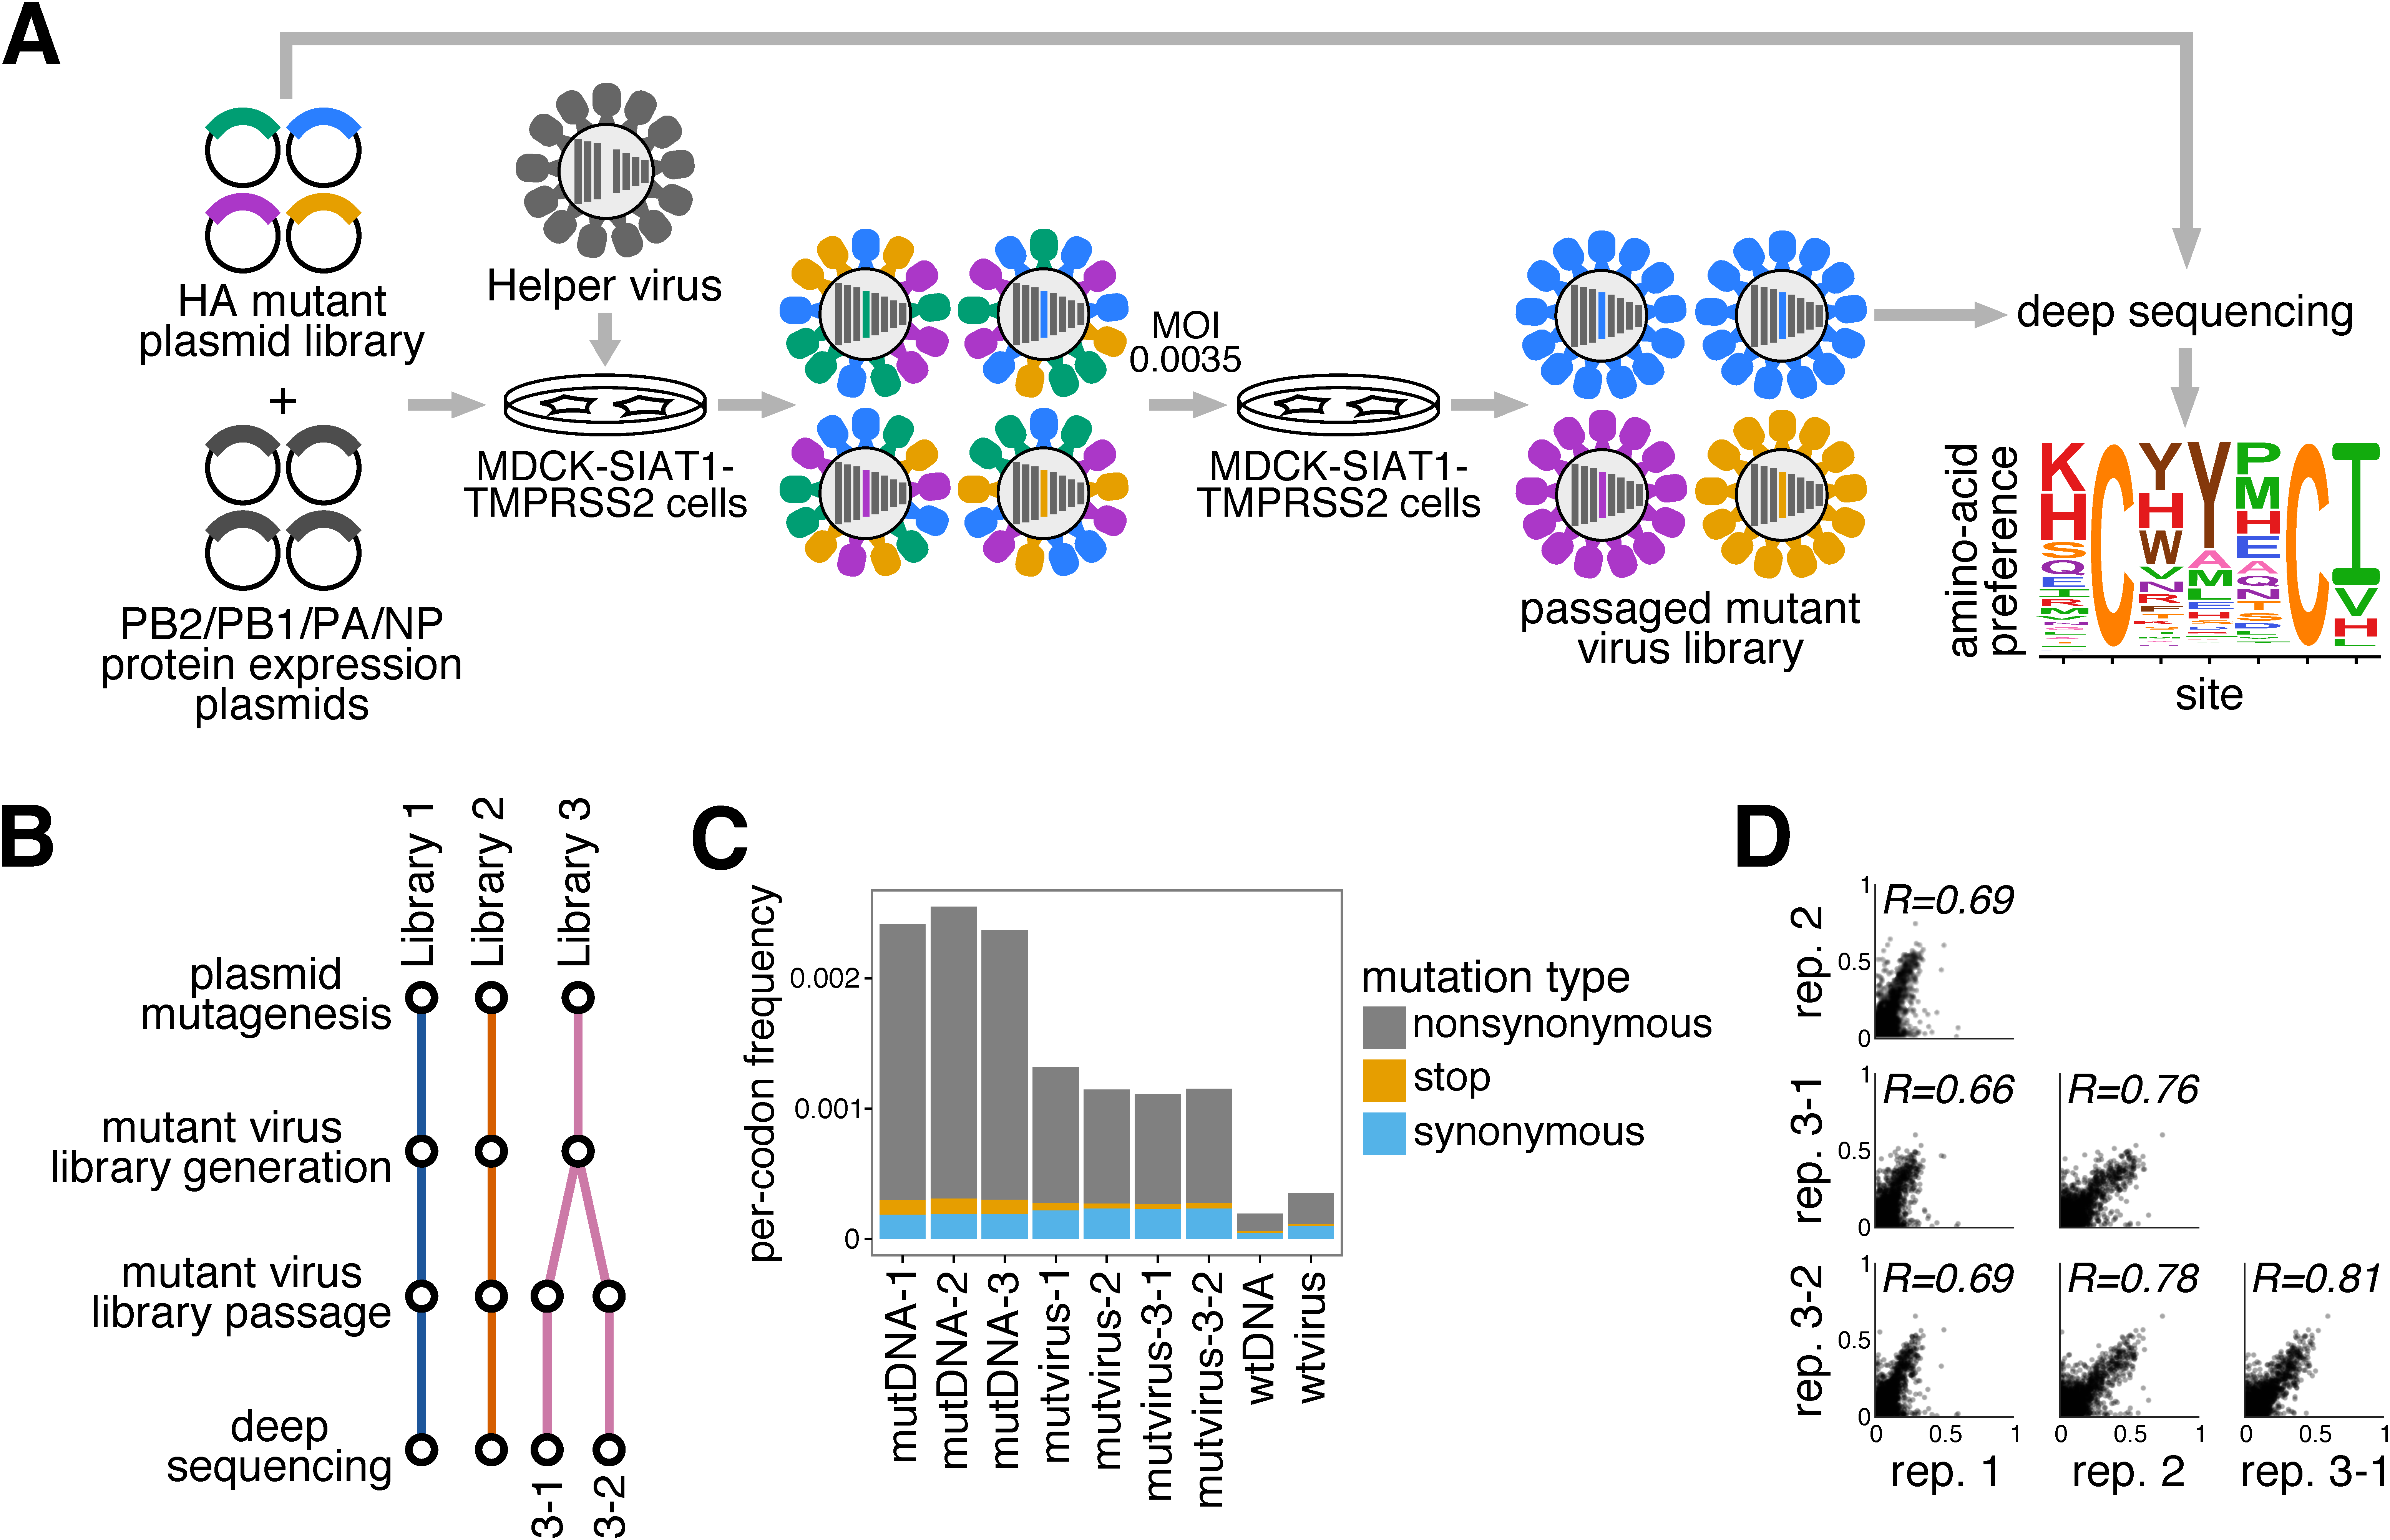
\includegraphics[width=\textwidth]{chapter_02/dms_overview.pdf}
  \caption[{Deep mutational scanning of the Perth/2009 H3 HA.}]{\label{fig:dms_overview}
    {\bf Deep mutational scanning of the Perth/2009 H3 HA.}
    (A) We generated mutant virus libraries using a helper-virus approach~\citep{Doud:2016gm}, and passaged the libraries at low MOI to establish a genotype-phenotype      linkage and to select for functional HA variants.
    Deep sequencing of the variants before and after selection allowed us to estimate each site's amino-acid preferences.
    (B) The experiments were performed in full biological triplicate.
    We also passaged and deep sequenced library 3 in duplicate.
    (C) Frequencies of nonsynonymous, stop, and synonymous mutations in the mutant plasmid DNA, the passaged mutant viruses, and wildtype DNA and virus controls.
    (D) The Pearson correlations among the amino-acid preferences estimated in each replicate.
  }
\end{figure}

Two main characteristics distinguish evolutionarily successful clades from their competitors: greater antigenic change, and efficient viral growth and transmission.
In principle, experiments could be informative for identifying how mutations affect these features.
Most work on influenza evolution to date has utilized experimental data to assess the antigenicity of circulating strains~\citep{sun2013using,harvey2016identification,Neher:2016hy,Koel:2013jz,Chambers:2015jt,li2016selection}.
However, the non-antigenic effects of mutations also play an important role~\citep{pybus2007phylogenetic,strelkowa2012clonal,Luksza:2014hj,Koelle:2015dh}.
Specifically, due to influenza virus's high mutation rate~\citep{holland1982rapid,steinhauer1987rapid,lauring2010quasispecies} and lack of intra-segment recombination~\citep{boni2008homologous}, deleterious mutations become linked to beneficial ones.
The resulting accumulation of deleterious mutations can affect non-antigenic properties central to viral fitness~\citep{Luksza:2014hj}.
However, there are no large-scale quantitative characterizations of how mutations to H3N2 HA affect viral growth.

It is now possible to use deep mutational scanning~\citep{fowler2014deep} to measure the functional effects of all single amino-acid mutations to viral proteins~\citep{Thyagarajan:2014go,Wu:2014ii,Doud:2016gm,haddox2016experimental,qi2015high,haddox2018mapping}.
However, the only HA for which such large-scale measurements have previously been made is from the highly lab-adapted A/WSN/1933 (H1N1) strain~\citep{Thyagarajan:2014go,Wu:2014ii,Doud:2016gm}.
Here, we measure the effects on viral growth in cell culture of all mutations to the HA of a recent human H3N2 strain.
We show that these experimental measurements can help discriminate evolutionarily successful mutations from those found in strains that quickly die out.
However, the utility of the experiments for understanding natural evolution depends on the similarity between the experimental and natural strains: measurements made on an H1 HA are less informative for understanding the evolutionary fate of H3 viral strains.

\section{Results}

\begin{figure}
\centering
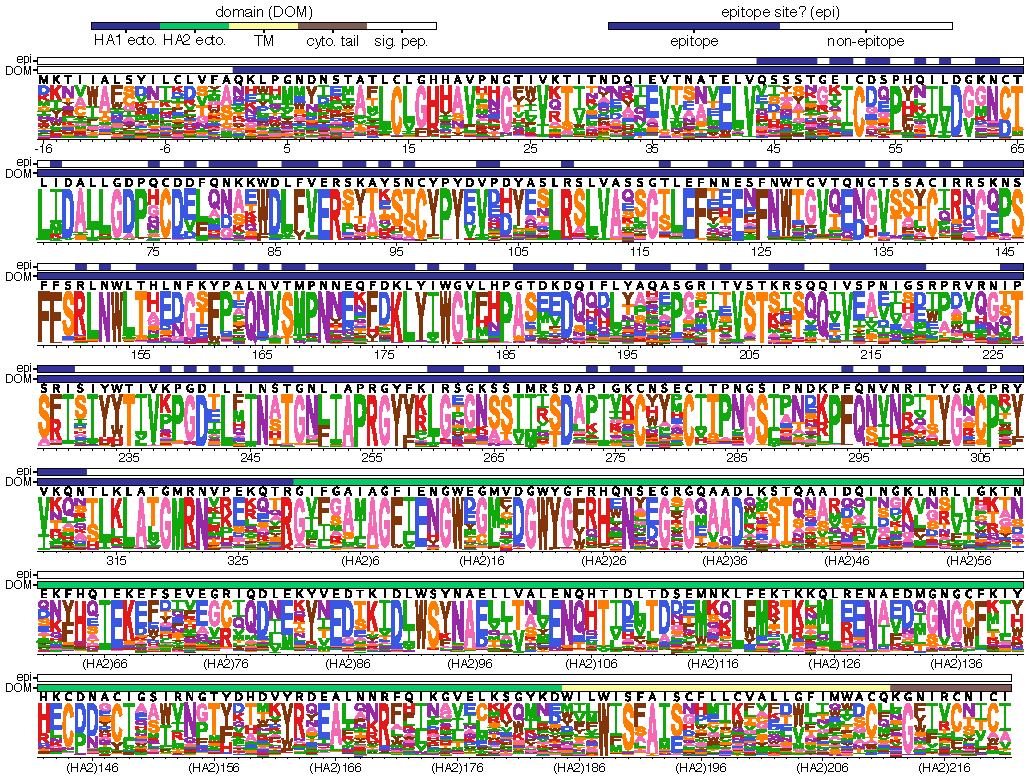
\includegraphics[width=\textwidth]{chapter_02/rescaled-avgprefs_prefs.pdf}
\caption[{The site-specific amino-acid preferences of the Perth/2009 HA measured in our experiments.}]{\label{fig:logoplot}
{\bf The site-specific amino-acid preferences of the Perth/2009 HA measured in our experiments.}
The height of each letter is the preference for that amino acid, after taking the average over experimental replicates and re-scaling~\citep{hilton2017phydms} by the stringency parameter in Table~\ref{tab:phydms}.
The sites are in H3 numbering.
The top overlay bar indicates whether or not a site is in the set of epitope residues delineated in \citet{Wolf:2006da}.
The bottom overlay bar indicates the HA domain (sig. pep. = signal peptide, HA1 ecto. = HA1 ectodomain, HA2 ecto. = HA2 ectodomain, TM = transmembrane domain, cyto. tail. = cytoplasmic tail).
The letters directly above each logo stack indicate the wildtype amino acid at that site.
}
\end{figure}

\subsection{Deep mutational scanning of HA from a recent strain of human H3N2 influenza virus}
We performed a deep mutational scan to measure the effects of all amino-acid mutations to HA from the A/Perth/16/2009 (H3N2) strain on viral growth in cell culture.
This strain was the H3N2 component of the influenza vaccine from 2010-2012~\citep{who2010d,who2011}.
Relative to the consensus sequence for this HA in Genbank, we used a variant with two mutations that enhanced viral growth in cell culture, G78D and T212I (see \citet{Lee2018} SI Appendix, Figure~S1 and Dataset~S1).
The G78D mutation occurs at low frequency in natural H3N2 sequences, and T212 is a site where a mutation to Ala rose to fixation in human influenza in $\sim$2011.

We mutagenized the entire HA coding sequence at the codon level to create mutant plasmid libraries harboring an average of $\sim$1.4 codon mutations per clone (see \citet{Lee2018} SI Appendix, Figure~S2).
We then generated mutant virus libraries from the mutant plasmids using a helper-virus system that enables efficient generation of complex influenza virus libraries~\citep{Doud:2016gm} (Figure~\ref{fig:dms_overview}A).
These mutant viruses derived all their non-HA genes from the lab-adapted A/WSN/1933 strain.
Using WSN/1933 for the non-HA genes reduces biosafety concerns, and also helped increase viral titers.
To further increase viral titers, we used MDCK-SIAT1 cells (Madin-Darby canine kidney cells overexpressing 2,6-sialyltransferase)~\citep{matrosovich2003overexpression} that we engineered to constitutively express TMPRSS2 (Transmembrane Protease, Serine 2), which cleaves the HA precursor to activate it for membrane fusion~\citep{bottcher2006proteolytic, bottcher2010cleavage}.

After generating the mutant virus libraries, we passaged them at low multiplicity of infection (MOI) in cell culture to create a genotype-phenotype link and select for functional HA variants (Figure~\ref{fig:dms_overview}A).
All experiments were completed in full biological triplicate (Figure~\ref{fig:dms_overview}B).
We also passaged and deep sequenced library 3 in duplicate (library 3-1 and 3-2) to gauge experimental noise \textit{within} a single biological replicate.
As a control to measure sequencing and mutational errors, we used the unmutated HA gene to generate and passage viruses carrying wildtype HA.

Deep sequencing of the initial plasmid mutant libraries and the passaged mutant viruses revealed selection for functional HA mutants.
Specifically, stop codons were purged to 20-45\% of their initial frequencies after correcting for error rates estimated by sequencing the wildtype controls (Figure~\ref{fig:dms_overview}C).
The incomplete purging of stop codons is likely because genetic complementation due to co-infection~\citep{marshall2013influenza, brooke2013most} enabled the persistence of some virions with nonfunctional HAs.
We also observed selection against many nonsynonymous mutations (Figure~\ref{fig:dms_overview}C), with their frequencies falling to 30-40\% of their initial values after error correction.

\begin{figure}
  \centering
  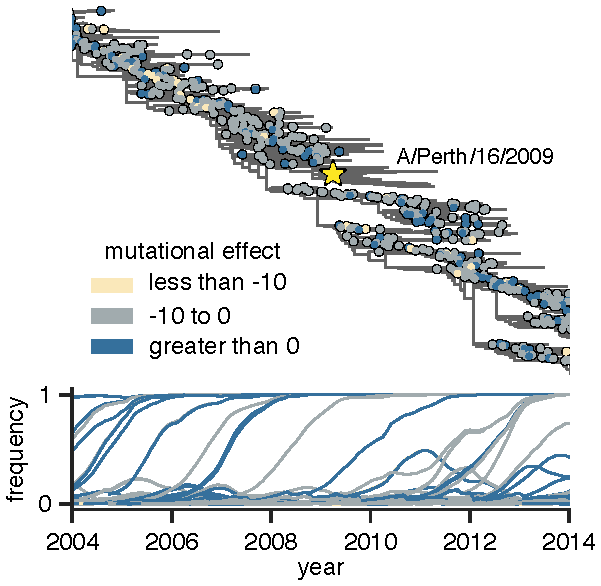
\includegraphics[width=0.75\textwidth]{chapter_02/frequency_trajectory_ex.pdf}
  \caption[{Frequency trajectories of individual mutations and their relation to the experimentally measured effects of these mutations.}]{\label{fig:frequency_trajectory}
    {\bf Frequency trajectories of individual mutations and their relation to the experimentally measured effects of these mutations.}
    The top panel shows the subset of the full H3N2 HA tree (Figure~\ref{suppfig:tree}) from 2004 to 2014.
    Circles indicate individual amino-acid mutations, and are colored according to the mutational effect measured in our deep mutational scanning (negative values indicate mutations measured to be deleterious to viral growth).
    The Perth/2009 strain is labeled with a star, and nodes in the clade containing the Perth/2009 strain were excluded from our analyses.
    The bottom panel shows the frequency trajectory of each mutation, with trajectories colored according to the mutational effects as in the top panel.
    It is clear that most mutations that reach high frequency are measured to be relatively favorable in our experiments.
    Figure~\ref{suppfig:head_stalk_mutfreq_supp} shows a similar layout but colors mutations by whether they are in HA's head or stalk domain.
}
\end{figure}

\subsection{Our measurements can help distinguish between mutations that reach low and high frequencies in nature}
Mutations occurring in the H3N2 virus population experience widely varying evolutionary fates (Figure~\ref{fig:frequency_trajectory}).
Some mutations appear, spread and fix in the population, while others briefly circulate before disappearing.
We take the maximum frequency reached by a mutation as a coarse indicator of its effect on fitness, since favorable mutations generally reach higher frequencies than unfavorable ones~\citep{ewens2012mathematical}.
Here, we follow the population genetic definition of \textit{mutation} and track the outcome of each individual mutation event, e.g.\ although R142G occurs multiple times on the phylogeny we track each of these mutations occurring on different backgrounds separately.
As such, each mutation is shown as a separate circle on a separate branch in Figure \ref{fig:frequency_trajectory}.
However, because multiple mutations on the same phylogeny branch cannot be disentangled, when multiple mutations occurred on a single branch, we assigned a single mutational effect based on the sum of effects of each mutation.

\begin{figure}
\centerline{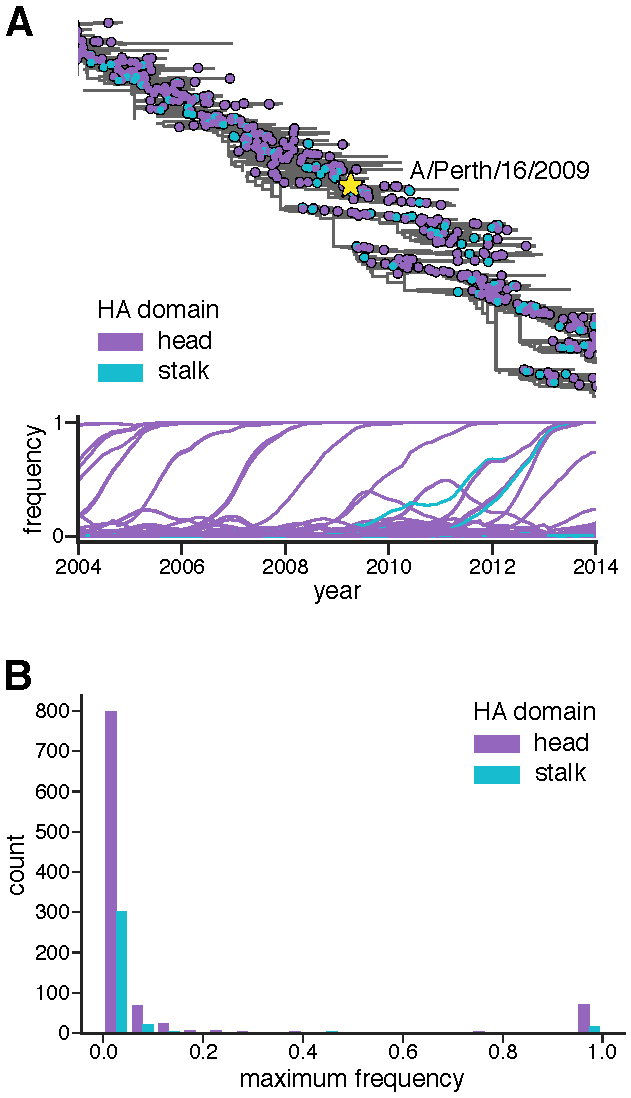
\includegraphics[width=0.55\textwidth]{chapter_02/head_stalk_mutfreq.pdf}}
\caption[{Frequency trajectories of head and stalk domain mutations.}]{\label{suppfig:head_stalk_mutfreq_supp}
{\bf Frequency trajectories of head and stalk domain mutations.}
(A) This figure repeats the analysis of the H3N2 mutation frequencies in Figure~\ref{fig:frequency_trajectory}, but colors amino-acid mutations by whether they occur in the head (purple) or the stalk (blue) domain.
(B) Histogram of mutation maximum frequencies by the number of mutations in the head and stalk domains.
It is clear that mutations in the head domain are more numerous than those in the stalk, particularly among mutations that reach high frequencies.
}
\end{figure}

After annotating mutations and their frequencies on the phylogeny in this way (Figure~\ref{fig:frequency_trajectory}), it is visually obvious that there are relatively few circulating mutations that we measure to be strongly deleterious---and that such deleterious mutations rarely reach high frequency when they do occur.

\begin{figure}
  \centering
  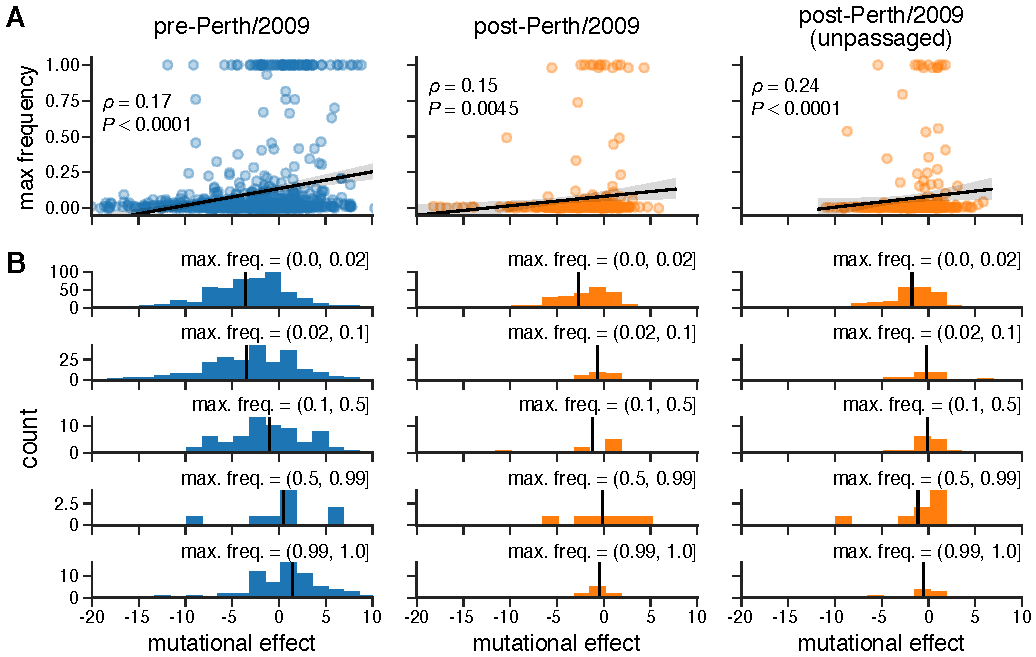
\includegraphics[width=\textwidth]{chapter_02/muteffect_by_maxfreq.pdf}
  \caption[{Experimental measurements are informative about the evolutionary fate of viral mutations.}]{\label{fig:muteffect_maxfreq}
    {\bf Experimental measurements are informative about the evolutionary fate of viral mutations.}
    (A) Correlation between the effects of mutations as measured in our deep mutational scanning of the Perth/2009 HA and the maximum frequency reached by these mutations in nature.
    The plots show Spearman $\rho$ and an empirical $P$-value representing the proportion of 10,000 permutations of the experimental measurements for which the permuted $\rho$ was greater than or equal to the observed $\rho$.
    (B) The distribution of mutational effects partitioned by maximum mutation frequency.
    The vertical black line shows the mean mutation effect for each category.
    The analysis is performed separately for pre-Perth/2009, post-Perth/2009, and unpassaged isolates from the post-Perth/2009 partitions of the tree (Figure~\ref{suppfig:tree}).
}
\end{figure}

We next sought to quantify the correlation between a mutation's experimentally measured effect and the maximum frequency it attained during natural evolution.
To calculate a given mutation's effect, we simply took the logarithm of the ratio of the preferences for the mutant and wildtype amino acids at that site.
To minimize effects related to the genetic background of the strain used in the experiment, we excluded mutations closely related to the experimental strain itself and partitioned the remaining mutations into 1,022 mutations pre-dating and 299 mutations post-dating the Perth/2009 strain (Figure~\ref{suppfig:tree}).
We additionally excluded mutations from the post-Perth partition that were sampled in 2014 or after, since these mutations have not had enough time for their evolutionary fates to be fully resolved.
We used these pre-Perth and post-Perth partitions to test the utility of our measurements for both post-hoc and prospective analyses, respectively.
We quantified the relationship between mutational effects and maximum mutation frequencies in the H3N2 phylogeny via Spearman rank correlation (Figure~\ref{fig:muteffect_maxfreq}A).
In both pre-Perth and post-Perth time periods, we found a modest, but statistically significant relationship between mutational effect and maximum mutation frequency (pre-Perth $\rho = 0.17$, post-Perth $\rho = 0.15$).
The similar effect sizes for both the pre- and post-Perth partitions shows that our experimental measurements can help explain the evolutionary fates of mutations in strains that post-date the experimentally studied strain, as well as to retrospectively analyze mutations that precede the experimental strain.

Many of the HAs in sequence databases are from viral isolates that were passaged in cell-culture or eggs, which can cause lab-adaptation mutations that confound evolutionary analyses~\citep{McWhite:2016fe}.
To check that our results were robust to such lab-adaptation mutations, we repeated our analysis using only HA sequences derived from viruses that had not been passaged in the lab.
Because sequencing of unpassaged primary isolates has only recently become commonplace, we could only perform this analysis for the post-Perth partition of the phylogenetic tree.
Figure~\ref{fig:muteffect_maxfreq}A shows that the correlation between our measured mutational effects and the maximum frequency was even stronger for mutations from unpassaged viral isolates ($\rho = 0.24$).

The trends in Figure~\ref{fig:muteffect_maxfreq}A are most strongly driven by the behavior of substantially deleterious mutations.
We investigated this further by partitioning mutations into those that reach low, medium and high frequencies, and those that fix in the population (Figure~\ref{fig:muteffect_maxfreq}B).
The mutations that reach higher frequencies have a more favorable mean effect.
Mutations measured to be substantially deleterious almost never reach high frequency.
Overall, these results demonstrate that measurements of how mutations affect viral growth in cell culture are informative for understanding the fates of these mutations in nature: in particular, if a mutation is measurably deleterious to viral growth, that mutation is unlikely to prosper in nature.

\begin{figure}
  \centering
  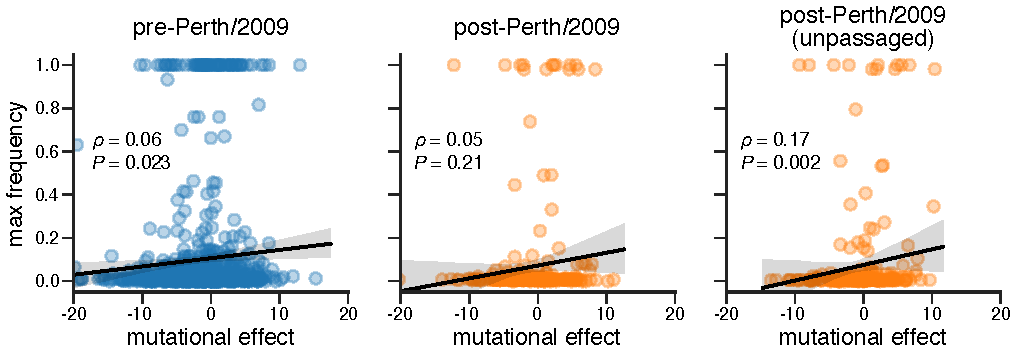
\includegraphics[width=\textwidth]{chapter_02/muteffect_by_maxfreq_WSN.pdf}
  \caption[{Experimental measurements on an H1 HA are less informative about the evolutionary fate of H3N2 mutations.}]{\label{fig:muteffect_maxfreq_WSN}
    {\bf Experimental measurements on an H1 HA are less informative about the evolutionary fate of H3N2 mutations.}
    This figure repeats the analysis of the H3N2 mutation frequencies in Figure~\ref{fig:muteffect_maxfreq}A, but uses the deep mutational scanning data for an H1 HA as measured in \citep{Doud:2016gm}.
    Figure~\ref{suppfig:muteffect_maxfreq_WSN_supp} shows the histograms comparable to those in Figure~\ref{fig:muteffect_maxfreq}B.
    The empirical $P$-value represents the result of 1,000 permutations.
  }
\end{figure}

\begin{figure}
\centerline{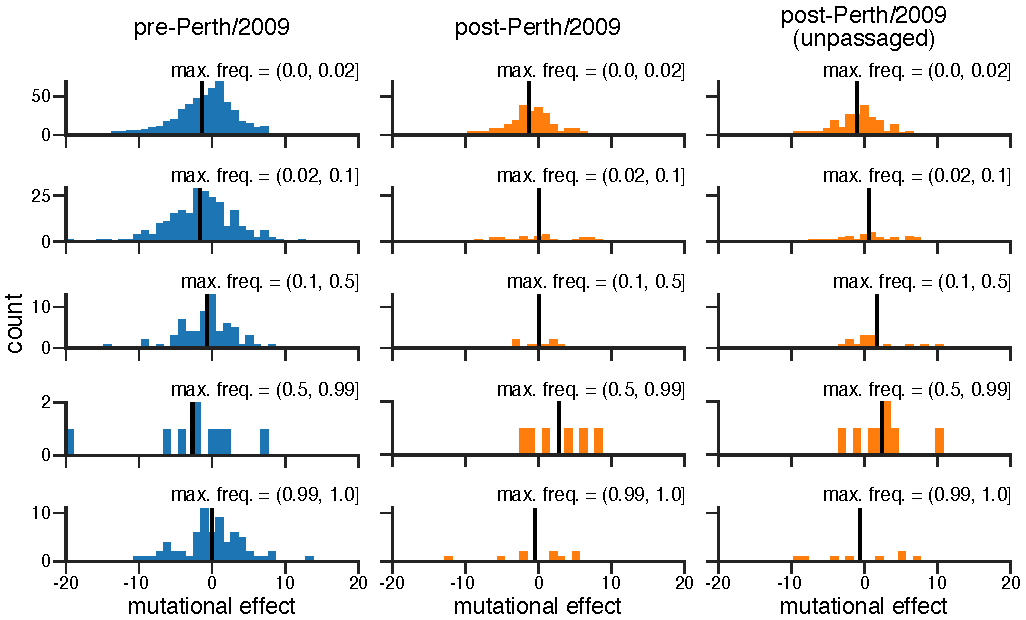
\includegraphics[width=\textwidth]{chapter_02/muteffect_maxfreq_WSN_supp.pdf}}
\caption[{The distribution of mutational effects measured in H1 HA among H3N2 mutations binned by the maximum frequency that they reach.}]{\label{suppfig:muteffect_maxfreq_WSN_supp}
{\bf The distribution of mutational effects measured in H1 HA among H3N2 mutations binned by the maximum frequency that they reach.}
This figure repeats the analysis of the H3N2 mutation frequencies in Figure~\ref{fig:muteffect_maxfreq}B, but uses the deep mutational scanning data for an H1 HA as measured in \citet{Doud:2016gm}.
}
\end{figure}

\subsection{Measurements made on an H1 HA are less informative for understanding the evolution of H3 influenza}
To determine how broadly experimental measurements can be generalized across HAs, we repeated the foregoing analysis of H3N2 mutation frequencies, but using mutational effects measured in our prior deep mutational scanning of the WSN/1933 H1 HA~\citep{Doud:2016gm} (see \citet{Lee2018} SI Appendix, Figure~S9), which is highly diverged from the Perth/2009 H3 HA (the two HAs only have 42\% protein sequence identity).
Figure~\ref{fig:muteffect_maxfreq_WSN} shows that the correlations between the H1 experimental measurements and the maximum frequency that mutations reach during H3N2 viral evolution are consistently weaker than those using H3 experimental measurements (compare Figure~\ref{fig:muteffect_maxfreq_WSN} to Figure~\ref{fig:muteffect_maxfreq}A).
Therefore, the utility of an experiment for understanding natural evolution degrades as the experimental sequence becomes more diverged from the natural sequences that are being studied.

\section{Discussion}
\label{sec:discussion}

We have measured the effects of all possible single amino-acid mutations to the Perth/2009 H3 HA on viral growth in cell culture and demonstrated that these measurements have some value for understanding the evolutionary fate of these mutations in nature.
Specifically, mutations measured to be more beneficial for viral growth tend to reach higher frequencies in nature than mutations measured to be more deleterious for viral growth.
The fact that our experiments can help identify evolutionary successful mutations suggests that they might inform evolutionary forecasting.
In their landmark paper introducing predictive viral fitness models that accounted for both antigenic and non-antigenic mutations, \citet{Luksza:2014hj} noted that the models could in principle be improved by integrating ``diverse genotypic and phenotypic data'' that more realistically represented the effects of specific mutations.
Our work suggests that deep mutational scanning may be able to provide such data.

It is important to emphasize that measurements of viral growth in cell culture do \emph{not} represent true fitness in nature.
Indeed, a vast amount of work in virology has chronicled the ways in which experiments can select for lab artifacts or fail to capture important pressures that are relevant in nature~\citep{daniels1985fusion,sun2010modifications,lee2013comparison,wu2017structural}.
As an example, although we identified G78D as favorable for viral growth in cell culture, this mutation never fixes in nature.
Mutations in viral genes other than HA are also important in determining strain success~\citep{memoli2009recent,raghwani2017selection}.
Given these caveats, it might seem surprising that measuring viral growth in cell culture can be informative about the success of viral strains in nature.
Yet, prior to our work, there were no comprehensive studies of the functional effects of mutations to H3 HA on any property that even resembled viral fitness in nature, and modeling work has either omitted the non-antigenic effects of mutations~\citep{sun2013using,harvey2016identification,Neher:2016hy} or assumed that all non-epitope mutations had equivalent deleterious effects~\citep{Luksza:2014hj}.
The strength of our measurements are not that they perfectly capture fitness in nature, but that they are systematic and quantitative---and so represent an improvement over no information at all.
We suspect that performing similar experiments using more realistic and complex selections (e.g., ferrets or primary human airway cultures) might further improve their utility and possibly their generalizability to more divergent strains.

We measured the effects of all single amino-acid mutations to a specific HA, and then generalized these measurements to other H3N2 HAs from a 50-year timespan.
These generalizations will only be valid to the extent that the effects of mutations are conserved during HA's evolution.
Extensive prior work has shown that epistasis can shift the effects of mutations as proteins evolve~\citep{pollock2012amino,shah2015contingency,gong2013stability,natarajan2013epistasis,harms2014historical,starr2016epistasis,starr2017alternative}.
Our work suggests that measurements on a HA from single human H3N2 viral strain can be usefully generalized to at least some extent across the entire evolutionary history of human H3N2 HA.
On the other hand, when we compared our measurements for an H3 HA to prior measurements on H1 HA, we found substantial shifts at many sites---much greater than those observed in prior protein-wide comparisons of more closely related homologs~\citep{doud2015site,haddox2018mapping}.
Further investigation of how mutational effects shift as proteins diverge will be important for determining how broadly any given experiment can be generalized when attempting to make evolutionary forecasts.

Our work did not characterize the antigenic effects of mutations, which also play an important role in determining strain success in nature~\citep{Koel:2013jz,Neher:2016hy}.
However, our basic selection and deep-sequencing approach can be harnessed to completely map how mutations affect antibody recognition~\citep{Doud:2017bw,doud2018quantifying}.
But so far, experiments using this approach have not examined antibodies or sera that are relevant to driving the evolution of H3N2 influenza~\citep{Doud:2017bw,doud2018quantifying}, or have used relevant sera but examined a non-comprehensive set of mutations~\citep{li2016selection}.
Future experiments that completely map how HA mutations affect recognition by human sera seem likely to be especially fruitful for informing viral forecasting.

\section{Materials and Methods}

\subsection*{Data and computer code}
Deep sequencing data are available from the Sequence Read Archive under BioSample accessions SAMN08102609 and SAMN08102610.
Computer code used to analyze the data is at \url{https://github.com/jbloomlab/Perth2009-DMS-Manuscript}.

\subsection*{HA numbering}
Sites are in H3 numbering, with the signal peptide in negative numbers, HA1 in plain numbers, and HA2 denoted with "(HA2)". Sequential 1, 2, ... numbering of the Perth/2009 HA can be converted to H3 numbering by subtracting 16 for the HA1 subunit, and subtracting 345 for the HA2 subunit.

\subsection*{Quantification of mutational effects}
The effect of mutating site $r$ from amino acid $a_1$ to $a_2$ was quantified as
\begin{equation}
\label{eq:muteffect}
\log_2 \frac{\pi_{r,a_2}}{\pi_{r,a_1}}
\end{equation}
where $\pi_{r,a_1}$ and $\pi_{r,a_2}$ are the re-scaled preferences for amino acids $a_1$ or $a_2$ at site $r$ as shown in Figure~\ref{fig:logoplot}.
The WSN/1933 H1 HA amino-acid preferences are the replicate-average values reported in \citep{Doud:2016gm}, re-scaled by a stringency parameter of 2.05 (see \url{https://github.com/jbloomlab/dms_tools2/blob/master/examples/Doud2016/analysis_notebook.ipynb}).

\begin{table}
\caption[{Substitution models informed by the experiments describe HA's evolution better than traditional models.}]{\label{tab:phydms}
  {\bf Substitution models informed by the experiments describe HA's evolution better than traditional models.}
  Maximum likelihood phylogenetic fit to an alignment of human H3N2 HAs using ExpCM~\citep{hilton2017phydms}, ExpCM in which the experimental measurements are averaged across sites (site avg.), and M0 and M5 versions of the Goldman-Yang (GY94) model~\citep{yang2000codon}.
  Models are compared by Akaike information criterion (AIC)~\citep{posada2004model} computed from the log likelihood (LnL) and number of model parameters.
  The $\omega$ parameter is dN/dS for the Goldman-Yang models, and the relative dN/dS after accounting for the measurements for the ExpCM.
  For the M5 model, we give the mean followed by the shape and rate parameters of the gamma distribution over $\omega$.
}
\begin{center}
\begin{tabular}{cccccccc}
\hline
\bf{Model} & \bf{$\Delta$AIC} & \bf{LnL} & \bf{Stringency} & \bf{$\omega$}  \\ \hline
ExpCM & 0.0 & -8441 & 2.47 & 0.91 \\
GY94 M5 & 2094 & -9482 & -- & 0.36 (0.30, 0.84) \\
ExpCM, site avg. & 2501 & -9692 & 0.67 & 0.32 \\
GY94 M0 & 2536 & -9704 & -- & 0.31 \\
\hline
\end{tabular}
 \end{center}
\end{table}

\subsection*{Inference of human H3N2 phylogenetic tree and calculation of maximum mutation frequencies}

\begin{figure}
\centerline{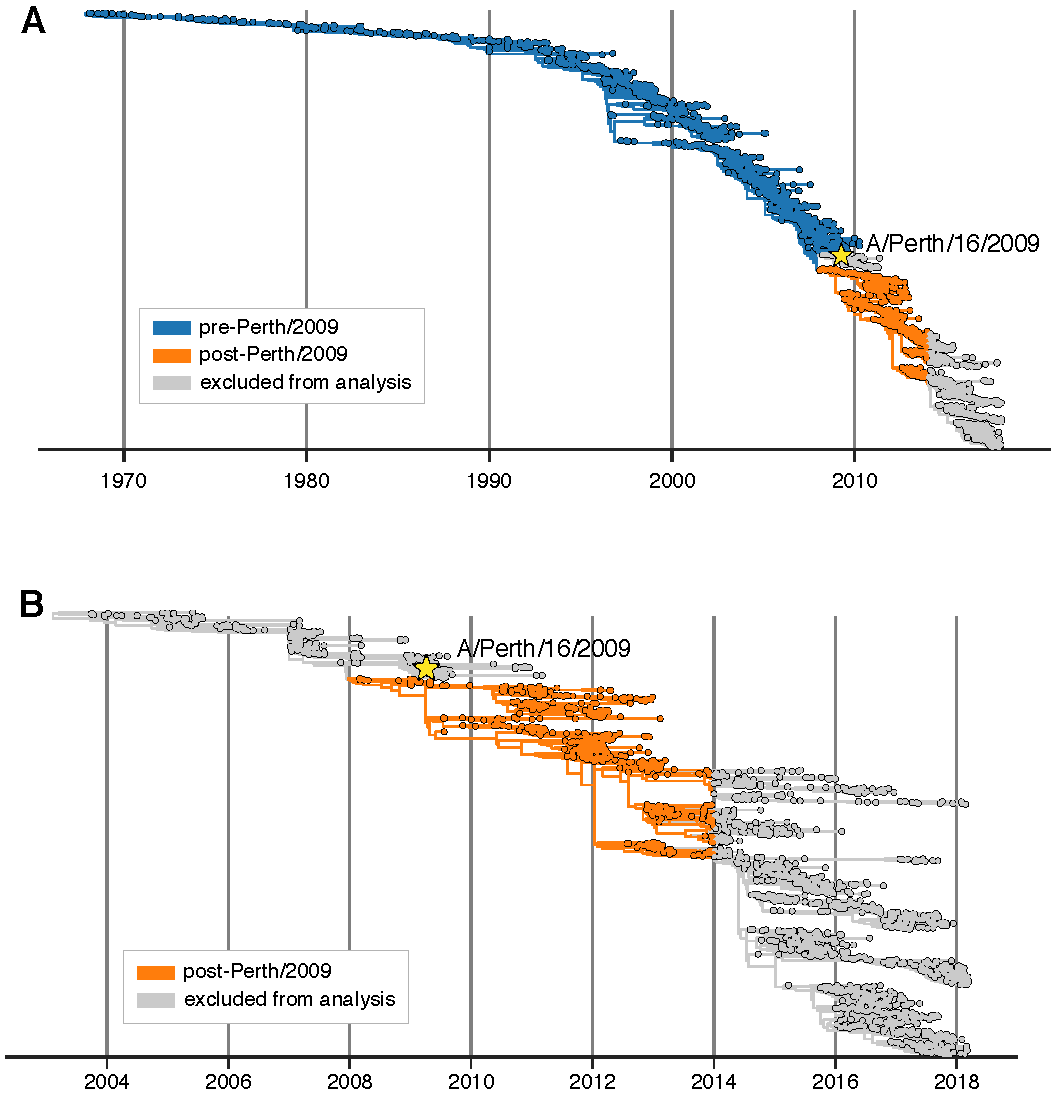
\includegraphics[width=\textwidth]{chapter_02/H3N2_phylogeny.pdf}}
\caption[{A phylogenetic tree of all HA sequences used in our analysis of mutation frequencies.}]{\label{suppfig:tree}
  {\bf A phylogenetic tree of all HA sequences used in our analysis of mutation frequencies.}
  (A) HA sequences were sampled at a rate of six viruses per month from January 1, 1968 through February 1, 2018.
  The Perth/2009 strain used in our experiments is indicated.
}
\end{figure}

\begin{figure}\ContinuedFloat
  \caption[{}]{(continued)
    The rest of the tree is partitioned into nodes that preceded the split of the Perth/2009 strain from the trunk of the tree (blue) and nodes that branched off the trunk after the clade containing Perth/2009 (orange).
    In Figure~\ref{fig:muteffect_maxfreq}, these two partitions of the tree are analyzed separately.
    Nodes in the clade containing the Perth/2009 strain and nodes sampled in 2014 or after were excluded from our analyses.
    The Perth/2009 strain was excluded to avoid artifacts related to mutations that occurred on the branches leading to the HA sequence used in the experiment.
    The post-2014 nodes were excluded because the evolutionary fates of many sequences after this date are not yet fully resolved.
    (B) The post-Perth/2009 partition of the tree containing only sequences from unpassaged isolates.
  }
\end{figure}

To generate the tree (Figure~\ref{suppfig:tree}), we applied Nextstrain's augur pipeline~\citep{Hadfield2018} (\url{https://github.com/nextstrain/augur}; commit \texttt{006896d}) to publicly available H3N2 HA sequences from GISAID \citep{shu2017gisaid} (see \citet{Lee2018} SI Appendix, Dataset~S4), sampling six viruses per month over the time interval of January 1, 1968 to February 1, 2018.
We aligned the resulting 2,189 HA sequences with MAFFT v7.310~\citep{katoh2013mafft} and constructed a maximum likelihood phylogeny from this alignment with RAxML 8.2.10~\citep{stamatakis2006raxml}.
Ancestral state reconstruction and branch length timing were performed with TreeTime~\citep{Sagulenko2018}.
The phylogenetic tree is available as a JSON file on GitHub at \url{https://github.com/jbloomlab/Perth2009-DMS-Manuscript/blob/master/analysis_code/data/flu_h3n2_ha_1968_2018_6v_tree.json.gz}.
The tree was visualized using BALTIC (\url{https://github.com/blab/baltic}).

% notation for frequencies model
\newcommand{\dx}{\mathrm{d}x}						% change in x
\newcommand{\dy}{\mathrm{d}y}						% change in y
\newcommand{\dt}{\mathrm{d}t}						% change in t
\newcommand{\inertia}{\epsilon}			    % inertia parameter
\newcommand{\normal}{\mathcal{N}}				% normal distribution

The frequency trajectory of each individual mutation on the phylogeny is estimated following Nextstrain's augur pipeline and as first implemented in Nextflu \citep{Neher:2015jr}.
Herein, mutation frequency dynamics are modeled according to a Brownian motion diffusion process discretized to one-month intervals.
The number of viruses sampled in each interval determines the denominator of the mutation frequency calculations.
Relative to a simple Brownian motion, the expectation includes an ``inertia'' term $\inertia$ that adds velocity to the diffusion and the variance includes a term $x(1-x)$ to scale variance according to frequency following a Wright-Fisher population genetic process.
This results in the following diffusion process
\begin{equation}
x(t+\dt) = \normal\big( x(t) + \inertia \, \dx , \; \dt \, \sigma^2 \, x(t) \, (1-x(t)) \big),
\end{equation}
with `volatility' parameter $\sigma^2$.
The term $\dx$ is the increment in the previous timestep, so that $\dx = x(t) - x(t-\dt)$.
We used $\inertia = 0.7$ and $\sigma^2 = 0.05$ to maximize fit to empirical trajectory behavior.

We also include an Bernoulli observation model for mutation presence / absence among sampled viruses at timestep $t$.
This observation model follows
\begin{equation}
f(x,t) = \prod_{v\in V} x(t) \prod_{v\notin V} (1-x(t)),
\end{equation}
where $v\in V$ represents the set of viruses that have the mutation and $v\notin V$ represents the set of viruses that do not have the mutation.
Each frequency trajectory is estimated by simultaneously maximizing the likelihood of the process model and the likelihood of the observation model via adjusting frequency trajectory $\mathbf{x}=(x_1, \ldots, x_n)$.

We also repeated the above analyses using only viruses that were sequenced directly without passaging.
Routine direct sequencing did not begin until the early 2000s \citep{McWhite:2016fe}.
To construct a tree with a similar number of viruses as the original analysis, we sampled 30 viruses per month between January 1, 2000 and April 1, 2018, producing a tree with 2,374 unpassaged viruses with augur (commit: \texttt{6d9f708}).
We included the passaged DMS strain, A/Perth/16/2009, in the resulting tree to enable comparison between pre-Perth and post-Perth clades.

\subsection{Analysis of full-length sequence preferences}
\label{subsec:sequence-preferences}

\begin{figure}
  \centering
  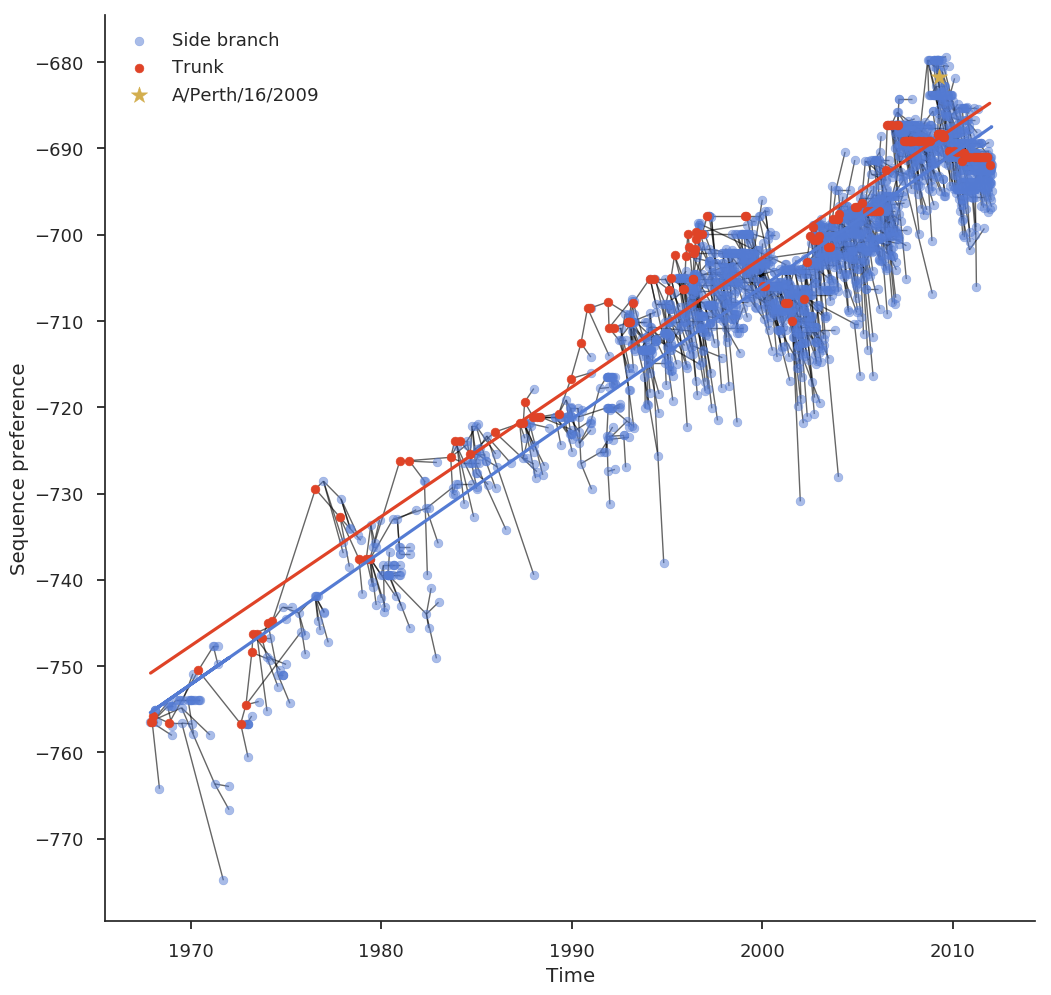
\includegraphics[width=\textwidth]{chapter_02/sequence-preference-per-strain-by-time-and-trunk-status.png}
  \caption[{Sequence preference by time for sequences from 1968--2012.}]{\label{fig:sequence-preference-per-strain} {\bf Sequence preference by time for sequences from 1968--2012.}
    Least squares regression lines are shown for trunk (red) and side branch (blue) nodes.
    The trunk line corresponds to the equation $y = 1.54x - 3779.83$ with an adjusted R-squared value of 0.87 ($p << 0.01$).
    The side branch line corresponds to the equation $y = 1.50x - 3700$ with an adjusted R-squared value of 0.88 ($p << 0.01$).
    The differences between these two equations is effectively eliminated when the same analysis is performed without terminal nodes.}
\end{figure}

We attempted to quantify the fitness of each H3N2 strain's complete HA sequence by summing the mutational preferences defined in Equation~\ref{eq:muteffect} across all positions in HA.
We anticipated that in the absence of epistasis the resulting sums would provide a metric of each strain's fitness with respect to its functional constraints.
Importantly, the sequence preference metric should also provide a fitness estimate that could be applied to any sequence without any additional phylogenetic information (i.e., the amino acid mutations present on branches leading to the strain in a phylogeny).

We calculated the sequence preference for all observed strains in the full phylogeny (Figure~\ref{suppfig:tree}) and their inferred ancestral sequences corresponding to internal nodes of the tree.
We additionally annotated each node of the tree by its status as belonging to the ``trunk'' or ``side branch'' of the phylogeny, using a previously published definition for these categories \citep{Bedford:2015fj}.
Nodes that belonged to the trunk category represent sequences that seeded future H3N2 populations while nodes on side branches failed to propagate.
We plotted the sequence preference of each node by its observed or inferred date and trunk status.

Surprisingly, we observed a positive linear trend for all sequences collected before the Perth/2009 strain (Figure~\ref{fig:sequence-preference-per-strain}).
This pattern reversed for all sequences collected after the Perth/2009 strain, showing a negative linear trend.
To better visualize and interpret these results, we fit linear regression models to both trunk and side-branch nodes and plotted the residuals for each sequence from the resulting models.
The residuals recapitulated the trends we observed in the sequence preferences by time and highlighted the greater divergence of trunk nodes from the positive linear trend after 2009 (Figure~\ref{fig:residuals-from-regression-fit-to-sequence-preference-per-strain}).
The same patterns appeared when we fit local weighted regression (LOWESS) lines to the residuals (Figure~\ref{fig:lowess-residuals-from-regression-fit-to-sequence-preference-per-strain})

\begin{figure}
  \centering
  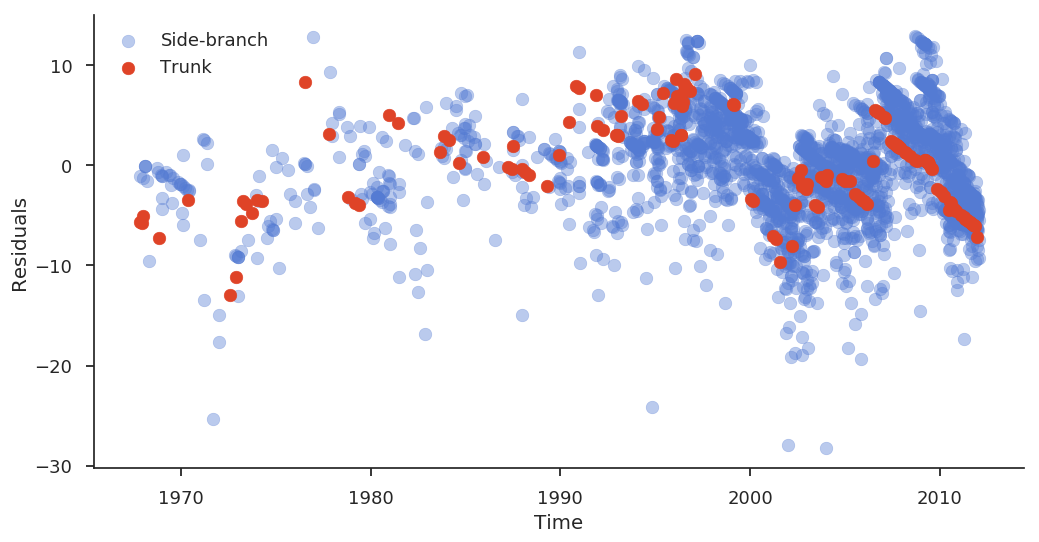
\includegraphics[width=\textwidth]{chapter_02/residuals-from-regression-to-sequence-preference-by-time-and-trunk-status.png}
  \caption[{Residuals by time based on linear regression equations in Figure~\ref{fig:sequence-preference-per-strain}.}]{\label{fig:residuals-from-regression-fit-to-sequence-preference-per-strain} {\bf Residuals by time based on linear regression equations in Figure~\ref{fig:sequence-preference-per-strain}.}
    The null expectation for the residuals is a horizontal line for both trunk and side-branch nodes with a trunk line slightly above the side-branch line.}
\end{figure}

\begin{figure}
  \centering
  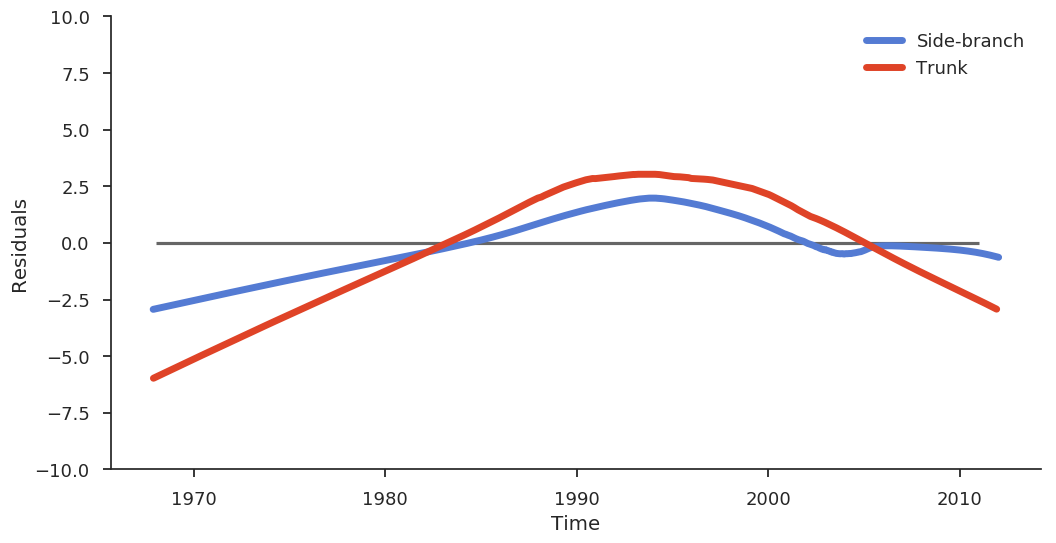
\includegraphics[width=\textwidth]{chapter_02/lowess-fit-to-residuals-from-regression-to-sequence-preference-by-time-and-trunk-status.png}
  \caption[{Local weighted regression (LOWESS) lines for trunk and side-branch residuals in Figure~\ref{fig:residuals-from-regression-fit-to-sequence-preference-per-strain}.}]{\label{fig:lowess-residuals-from-regression-fit-to-sequence-preference-per-strain} {\bf Local weighted regression (LOWESS) lines for trunk and side-branch residuals in Figure~\ref{fig:residuals-from-regression-fit-to-sequence-preference-per-strain}.}}
\end{figure}

From these results, we concluded that the sequence preference metric was strongly influenced by the genetic background of the DMS preferences themselves (i.e., the Perth/2009 strain).
We interpreted the positive linear trend toward the Perth/2009 era as a representation of H3 sequences that gradually accumulated mutations that made them appear more like the Perth/2009 strain.
This interpretation was supported by the fact that the Perth/2009 strain had one of the highest possible sequence preferences and therefore represented a kind of ``fitness peak'' for the sequence preference metric.
From the decline of sequence preferences after 2009 even for trunk nodes, we concluded that the sequence preference was not a reliable fitness metric for long-term forecasts of H3N2 evolution.
We resolved to use mutation-specific DMS preferences for the remainder of our analyses, to minimize the effects of epistasis on our results.
